
\chapter{Resolución del trabajo}
 
\section{Materiales}

\subsection{Familia Zynq-7000}

La familia \textbf{Zynq-7000} integra un sistema completo con un procesador \textit{ARM Cortex-A9 MPCore} con una lógica genérica que 
permite la configuración de módulos hardware específicos. Esta familia de SoCs está diseñada para llevar a cabo aplicaciones de compleja 
dificultad como la video-vigilancia o sistemas inalámbricos. 

El software de Xilinx \textbf{ISE} no estaba preparado para soportar la complejidad y capacidad de un diseño de una FPGA con un procesador 
ARM. \textit{Vivado Design Suite} (Figura \ref{vivadoGUI}) fue desarrollado para FPGAs con más capacidad y permite compilaciones de descripciones 
basadas en \(C\) gracias a la funcionalidad de síntesis de alto nivel.

\subsection{Tarjeta Zybo}

Una FPGA de la familia Zynq 7000 es incluida en tarjeta \textbf{ZYBO} (\textit{ZYbo BOard}). Es una plataforma de desarrollo de circuito 
digital, y está construida alrededor del miembro más pequeño de la familia Zynq-7000, el \textbf{Z-7010}. Se basa en la arquitectura 
\textbf{AP SoC} (\textit{Xilinx All Programmable System-on-Chip}), que integra un procesador 
de doble núcleo ARM Cortex-A9 con lógica \textit{Xilinx 7-series FPGA}.

La Zynq 7010 Ap SoC ofrece las siguientes características (Figura \ref{fig:zybo}) \cite{manual_zybo}:
\begin{itemize}
    \item Procesador dual-core Cortex-A9 de 650Mhz
    \item Controlador de memoria DDR3 con 8 canales DMA
    \item Controladores periféricos de alto ancho de banda: 1G Ethernet, USB 2.0, SDIO
    \item Controladores periféricos de bajo ancho de banda: SPI, UART, CAN, \(I^2C\)
    \item Lógica Reprogramable equivlente a Artix-7 FPGA
    \item ZYNQ XC7Z010-1CLG400C
    \item Puerto HDMI
    \item Puerto VGA de 16 bits por pixel
    \item EEPROM externo
    \item Códec de audio con salida de auricular y micrófono 
    \item GPIO: 6 botones, 4 interruptores, 5 LEDs
    \item 6 conectores Pmod
\end{itemize}

\begin{figure}
    \centering
    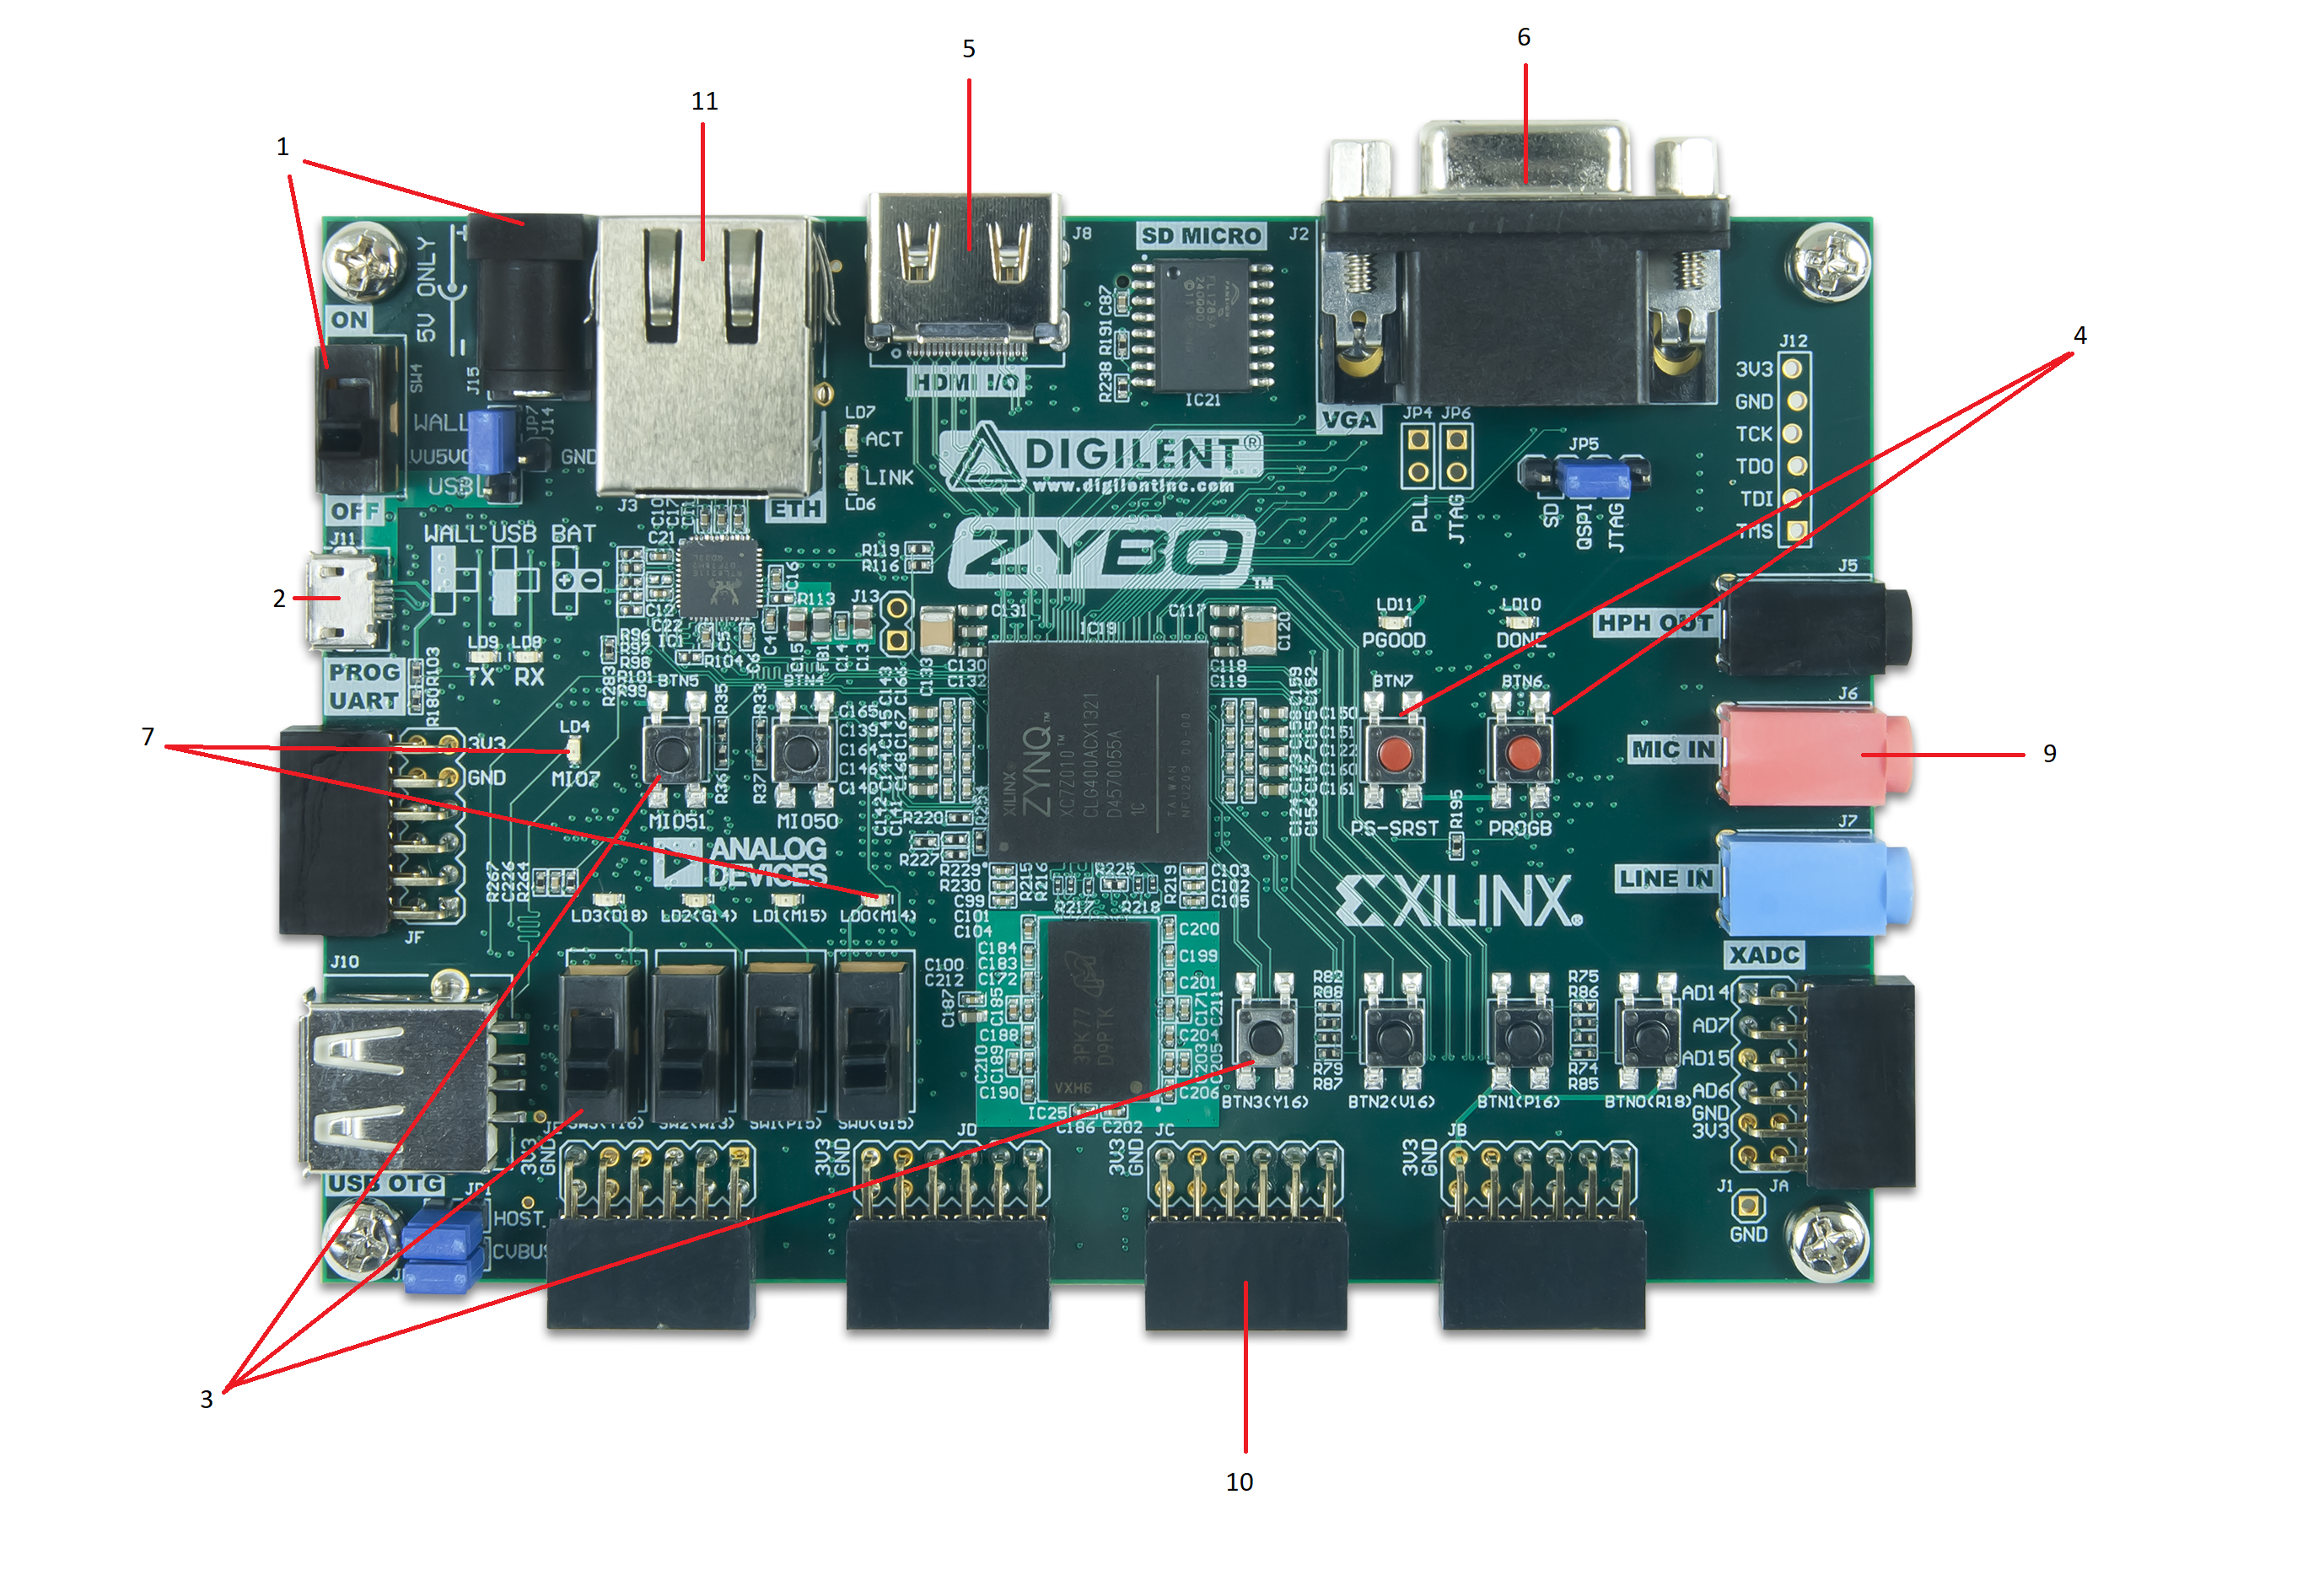
\includegraphics[width = 1\textwidth]{imagenes/zybo2.png}
    \caption{ZYBO Zynq-7000 Development Board}\label{fig:zybo}
\end{figure}

La arquitectura Zynq AP SoC está dividida en dos partes (Figura \ref{fig:zynq}), el sistema de procesamiento (\textit{PS}) y la lógica programable (\textit{PL}). 
La PL usada es parecida a la de la FPGA \textit{Xilinx 7-series Artix}, excepto porque contiene buses y puertos dedicados que hacen que esté 
acoplado fuertemente al PS. Además, la PL no tiene la misma configuración hardware como las FPGAs 7-series y tiene que ser configurada 
por el procesador o por el puerto JTAG.

\begin{figure}[H]
    \centering
    \includegraphics[width = 1\textwidth]{imagenes/zynqapsoc.png}
    \caption{Arquitectura Zynq AP SoC}\label{fig:zynq}
\end{figure}

El PS consiste en un conjunto de componentes como la \textit{APU} (Unidad de Procesamiento de Aplicaciones) que incluye dos procesadores Cortex-A9, 
\textit{AMBA} (Arquitectura de Bus de Microcontrolador Avanzada), Controlador de Memoria \textit{DDR3}, y varios controladores periféricos con 
las entradas y salidas multiplexadas a 54 pines dedicados (\textit{MIO}). Los controladores periféricos están conectados al procesador mediante 
la interconexión \textit{AMBA} y la PL está conectada de la misma manera.

Los elementos que forman la tarjeta Zybo son (Figura \ref{fig:zybo}):
\begin{enumerate}
    \item \textbf{Interruptor y Conector de alimentación}
    \item \textbf{Botones e interruptores} 
    \item \textbf{Botones de reset} 
    \item \textbf{Puerto HDMI} 
    \item \textbf{Puerto VGA} 
    \item \textbf{LEDs} 
    \item \textbf{Conectores de audio} 
    \item \textbf{Conectores Pmod} 
    \item \textbf{Conector Ethernet}
\end{enumerate}

La tarjeta Zybo incluye cuatro interruptores, cuatro botones y cuatro LEDs individuales a la PL. Además hay 2 botones y un LED conectados 
directamente al PS v¡a través de pines MIO. Adicionalmente hay un LED de encendido de la tarjeta, otros dos para el estado del puerto USB 
y un último LED para el estado de la programación de la FPGA.

Uno de los \textbf{botones de reset} reestablece la PL, que permanecerá sin configurar hasta ser reprogramado de nuevo. El otro reinicia 
el dispositivo sin afectar al entorno de depuración. 

Nos encontramos con tres \textbf{Conectores de audio}, dos entradas para micrófono y línea estéreo y una salida para auriculares.

El \textbf{Puerto VGA} (\textit{Video Graphics Array}) es una interfaz que recibe señal a través de un conector VGA. Éste se suele usar 
para conectar dispositivos. Está compuesto de 15 pines y cada uno tiene su propia función, entre las cuales está la de transferir los 
colores rojo, azul y verde, la sincronización horizontal y la sincronización vertical. 

El \textbf{Puerto HDMI} es un conector de entrada y salida con el que se puede transmitir vídeo compatible con HDMI o DVI. 

Los \textbf{Conectores Pmod} (\textit{Módulos Periféricos}) son unos conectores con estándares de módulos periféricos, para ampliar la capacidad de la 
lógica programable. Se comunican mediante 6,8 ó 12 pines para transportar señales de control digital. En nuestro caso, son 12 pines (2x6). 
Hay 6 conectores Pmod con distinto comportamiento en esta tarjeta y cada uno pertenece a una de las cuatro categorías, ``standard'', ``MIO connected'', 
``XADC'' y ``high-speed''.


\subsection{Vivado}

Zybo es compatible con \textit{Vivado Design Suite} de Xilinx así como con el conjunto de herramientas ISE/EDK.
Estas herramientas combinan el diseño lógico FPGA con el desarrollo software de ARM. Se pueden utilizar para diseñar sistemas 
de cualquier complejidad, desde un sistema operativo completo hasta un programa simple que controla algunos LEDs.

\textbf{Vivado Design Suite} es un entorno de diseño integrado (\textbf{IDE}) de Xilinx para la síntesis y análisis de diseños HDL. Vivado incluye 
su propio simulador lógico y además está la posibilidad de usar otros simuladores como \textit{ModelSim}, \textit{Mentor Questa}, 
\textit{Candence IES} o \textit{Synopsys VCS}. Además incluye síntesis a alto nivel con una herramienta que convierte código C a lógica
 programable.

Está formado por 4 componentes:
\begin{itemize}
    \item \textbf{Vivado High-Level Synthesis} - Permite usar programas en \(C\), \(C++\) y \(SystemC\) en dispositivos Xilinx  sin necesidad 
    de crear un RTL manualmente. Aumenta la productividad del desarrollador y admite clases, plantillas, funciones y sobrecarga de operadores.
    \item \textbf{Vivado Simulator} - Es un simulador controlado por eventos de lenguaje de descripción hardware (\textbf{HLD}) que admite 
    simulación de comportamiento y tiempos. Además admite scripts TCL (\textit{Tool Command Language}) en lenguaje mixto, es decir, admite
     lenguajes como \textit{Verilog}, \textit{SystemVerilog} y \textit{VHDL}.
    \item \textbf{Vivavo IP Integrator} - Permite integrar y  configurar IP (``\textit{Intellectual Property}") desde la biblioteca propia de Xilinx.
    \item \textbf{Vivado TCL Store} - Es un sistema de comandos para desarrollar complementos para Vivado además de agregar y modificar las 
    capacidades de Vivado. Todas las funciones de Vivado se pueden controlar con los scripts TCL.
\end{itemize}

En concreto, la versión que se ha utilizado es con Vivado 2016.2. Para trabajar con él, se puede hacer tanto trabajando con la TCL o 
directamente con la GUI de Vivado IDE \cite{vivadoIDE}. 
\begin{figure}[H]
    \centering
    \includegraphics[width = 1\textwidth]{imagenes/Vivado1.png}
    \caption{Vivado IDE}\label{vivadoGUI}
\end{figure}

La sección \textbf{Quick Start} nos proporciona fácil acceso a la creación de un nuevo proyecto, abrir proyectos existentes o abrir proyectos 
de ejemplo ofrecidos por Xilinx. Además, en la sección \textbf{Recent Projects} se pueden abrir proyectos usados recientemente.

En la sección \textbf{Tasks} encontramos el acceso a \textbf{Manage IP} que nos permite ver el catálogo de IP, personalizar IP y generar 
productos de salida.  \textbf{Open Hardware Manager} nos permite conectar la tarjeta y descargar un programa en el dispositivo FPGA. 
\textbf{Xilinx TCL Store} es un repositorio de código TCL. Da acceso a múltiples scripts para resolver problemas y mejorar la productividad.

La última sección es \textbf{Information Centre} donde se encuentra el acceso directo a la documentación, tutoriales y videos sobre lo que se 
puede hacer con esta herramienta.

Los componentes principales de la Figura \ref{vivado2} son:
\begin{enumerate}
    \item \textit{Menu Bar}
    \item \textit{Main Toolbar}
    \item \textit{Flow Navigator}
    \item \textit{Layout Selector}
    \item \textit{Data Windows Area}
    \item \textit{Workspace} 
    \item \textit{Menu Command Search Field} 
    \item \textit{Project Status Bar} 
    \item \textit{Results Windows Area}
\end{enumerate}

\begin{figure}[H]
    \centering
    \includegraphics[width = 1\textwidth]{imagenes/vivado2.png}
    \caption{Entorno Principal Vivado IDE}\label{vivado2}
\end{figure}

%\textit{Menu Bar} nos da acceso a los comandos de Vivado IDE. Normalmente, cuando se inicia un proyecto, no todos los comandos están 
%disponibles, sino que algunos se muestran cuando el diseño está activo.

%\textit{Menu Command Search Field} se encuentra a la derecha del anterior y permite localizar y ejecutar un comando de manera más rápida. La 
%lista de comandos que aparecen en la búsqueda están basados en el contexto del proyecto del diseño actual.

%\textit{Main Toolbar} nos da acceso a los comandos más usados en Vivado IDE. Si se pone el cursor en alguno de estos comandos, Vivado 
%ofrece más información acerca del mismo.

\textit{Flow Navigator} (Figura \ref{flownavigator}) permite acceder a comandos y herramientas que van desde abrir diseños a crear un archivo bitstream. Las 
diferentes secciones permiten hacer lo siguiente:
\begin{itemize}
    \item \textit{\textbf{Project Manager}}: Cambio de ajustes generales, añadir o crear archivos o abrir el Catálogo de IPs
    \item \textit{\textbf{IP Integrator}}: Crear, abrir o generar un bloque de diseño. 
    \item \textit{\textbf{Simulation}}: Cambio de ajustes de simulación o simular un diseño activo.
    \item \textit{\textbf{RTL Analysis}}: Abrir un diseño elaborado o generar un diseño de diagrama de circuitos RTL.
    \item \textit{\textbf{Synthesis}}: Cambio de ajustes de síntesis, sintetizar un diseño activo o abrir el diseño sintetizado.
    \item \textit{\textbf{Implementation}}: Cambio de ajuste de implementación, implementar un disñeo activo o abrir el diseño implementado.
    \item \textit{\textbf{Program and Debug}}: Cambio de ajustes del bitstream, generar un archivo bitstream o abrir una ventana para 
    conectar la tarjeta FPGA y programarla.
\end{itemize}

\begin{figure}[H]
    \centering
    \includegraphics[width = 0.5\textwidth]{imagenes/flownavigator.png}
    \caption{\textit{Flow Navigator}}\label{flownavigator}
\end{figure}

\textit{Layout Selector} proporciona el diseño de ventanas predefinidas para facilitar el proceso de diseño. Entre las opciones tenemos:
\begin{itemize}
    \item \textit{\textbf{Default Layout}}: Muestra el diseño con el mínimo número de ventanas, con un resumen global del diseño (Figura \ref{default}).
    \item \textit{\textbf{I/O Planning}}: Definición de restricciones de ubicación I/O y colocación de puertos (Figura \ref{io}).
    \item \textit{\textbf{Clock Planning}}: Planificación y colocación de los recursos del reloj del diseño (Figura \ref{clock}).
    \item \textit{\textbf{Floorplanning}}: Gestionar particiones y tareas jerárquicas (Figura \ref{fp}).
    \item \textit{\textbf{Timing Analysis}}: Ejecutar informes de tiempo y analizarlo (Figura \ref{ta}).
\end{itemize} 

\begin{figure}[H]
    \centering
    \includegraphics[width = 1\textwidth]{imagenes/default.png}
    \caption{\textit{Default Layout}}\label{default}
\end{figure}

\begin{figure}[H]
    \centering
    \includegraphics[width = 1\textwidth]{imagenes/io.png}
    \caption{\textit{I/O Planning}}\label{io}
\end{figure}

\begin{figure}[H]
    \centering
    \includegraphics[width = 1\textwidth]{imagenes/clock.png}
    \caption{\textit{Clock Planning}}\label{clock}
\end{figure}

\begin{figure}[H]
    \centering
    \includegraphics[width = 1\textwidth]{imagenes/fp.png}
    \caption{\textit{Floorplanning}}\label{fp}
\end{figure}

\begin{figure}[H]
    \centering
    \includegraphics[width = 1\textwidth]{imagenes/ta.png}
    \caption{\textit{Timing Analysis}}\label{ta}
\end{figure}

\textit{Project Status Bar} da información sobre el estado actual del diseño activo. \textit{Data Windows Area} muestra información 
sobre los archivos que forman el diseño. \textit{Workspace} muestra ventanas como el editor de textos o el diseño del diagrama de 
circuitos, entre otros. Y \textit{Results Windows Area} presenta los resultados de los comandos ejecutados. Además se muestran 
distintas ventanas, como \textit{Tcl Console}, \textit{Messages}, \textit{Log}, \textit{Reports} y \textit{Design Runs}.

\section{Metodología}

\section{Desarrollo de módulos hardware específicos}

\section{Casos prácticos}
